\subsection{Audio Engine des Samplers}

Die Hauptfunktionalität eines Audiosamplers ist natürlich das Aufnehmen und Abspielen von Audiosamples. 

Der ausgesuchte PCM5102a Audio Codec verfügt lediglich über einen Ausgabestream, was eine Neubestellung eines Codecs mit In- und Output Stream erfordern würde.

Angesichts des ohnehin schon ambitionierten Featureumfangs und der damit verbundenen Zeitknappheit, wurde die Aufnahmefunktion gestrichen, sodass der Prototyp zu einer reinen ``Sample-Playback`` Maschine wird. (TODO Verweis auf Lastenfall)

Das folgende Kapitel befasst sich mit der Implementierung und Ansteuerung der Audiowiedergabe über den Audio Codec und aller verbundenen DSP-Operationen.

Zunächst folgt eine Erläuterung des grundlegenden Signalfluss der Audioengine:

\subsubsection{Signalfluss der Audioengine}

Alle Audiosamples werden auf einer angeschlossen \textbf{SD Karte} persistent gespeichert. Diese werden dann immer stückweise mit dem \textbf{FATFS} Dateisystem, welches für eingebettete Systeme optimiert ist, in die Applikationslogik und somit den Audiopufferspeicher geladen. 

Von hier aus reicht die \textbf{DMA} den Buffer per \textbf{I2S} Protokoll an den \textbf{Audio Codec} weiter. 

Der Audio Codec wandelt die digitalen PCM Signale in eine analoges Signal mit Line-Level. %(TODO: Line Pegel elektrisch angeben). evtl auf Datenblatt verweisen?

\begin{figure}[h!]
	\centering
	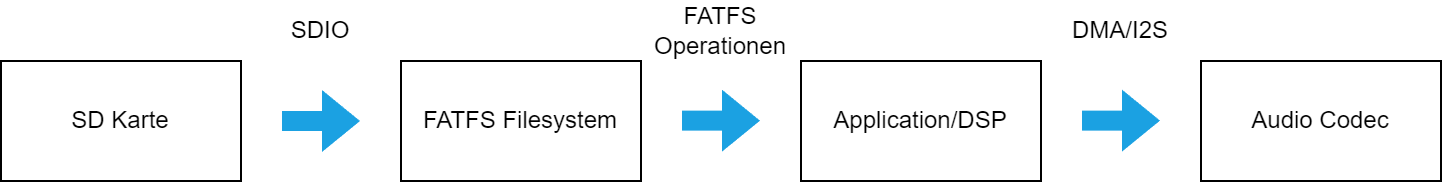
\includegraphics[width=0.9\textwidth]{images/08_durchfuehrung/audio/audio_signalflow.drawio.png}
	\caption{Digitaler Audio Signalfluss}
	\label{fig:audio_signalflow}
\end{figure}


\subsubsection{Latenzen}

%TODO: TEST MIT MESSUNG IN TESTS (pulse an gpio geben, und audioausgang mit osci messen)

Echtzeitfähigkeit ist ein kritischer Aspekt bei elektronischen Audioinstrumenten. 
Eine niedrige Latenz ist entscheidend, um rhythmisch präzise und ``tight`` zu spielen, besonders wenn mehrere Instrumente miteinander synchronisiert werden müssen.

Die maximale Latenz, die ein menschlicher Profimusiker noch akzeptieren kann, liegt bei etwa 20ms. Diese Richtwert basiert auf der Wahrnehmungsgrenze, bei der Musiker und Live-Performern keine signifikante zeitliche Verzögerung zwischen dem Triggern eines Samples und dessen tatsächlichem Output am Ausgang spüren (https://www.highfidelity.com/backlog/how-much-latency-can-live-musicians-tolerate-da8e2ebe587a)

Um die Latenz auf ein Minimum zu reduzieren und sicherzustellen, dass elektronische Audioinstrumente reaktionsschnell und synchronisiert sind, können folgende Methoden angewendet werden:

\paragraph{Dimensionierung der Buffersize}\

Die erste Stellschraube ist die \textit{Buffersize}.
Das ist die Größe (in Bytes) des Audiobuffers.
Je kleiner der Audiobuffer, desto öfter pro Sekunde gibt die DMA dessen Inhalt an den Audio Codec weiter.

Das bringt jedoch auch Performanceeinbußen mit sich: Bei kleinen Audiobuffern hat die CPU, je nach Komplexität der durchzuführenden DSP-Operationen, möglicherweise nicht genug Zeit, um den gesamten Buffer zu verarbeiten.
Ein nur teils verarbeiteter Buffer kann hörbare Knackser und Störgeräusche am Ausgangssignal verursachen.

Hier gilt es also, die kleinstmögliche Buffersize zu ermitteln, ohne dass Störgeräusche auftreten.
Nach Experimentieren hat sich ein Wert von \textbf{128 Bytes} als adäquat herausgestellt.

\paragraph{Verwendung von Double Buffering}\

Double Buffering ermöglicht es, Daten in einem Pufferspeicher zu verarbeiten, während gleichzeitig ein anderer Puffer für die Eingabe oder Ausgabe verwendet wird. Dies reduziert Verzögerungen und ermöglicht eine nahtlose Datenverarbeitung, da der Prozessor nicht auf das Ende einer Übertragung oder Berechnung warten muss, bevor er fortfahren kann. (Quelle: https://www.eetimes.com/fundamentals-of-embedded-audio-part-3/)

\begin{figure}[H]
	\centering
	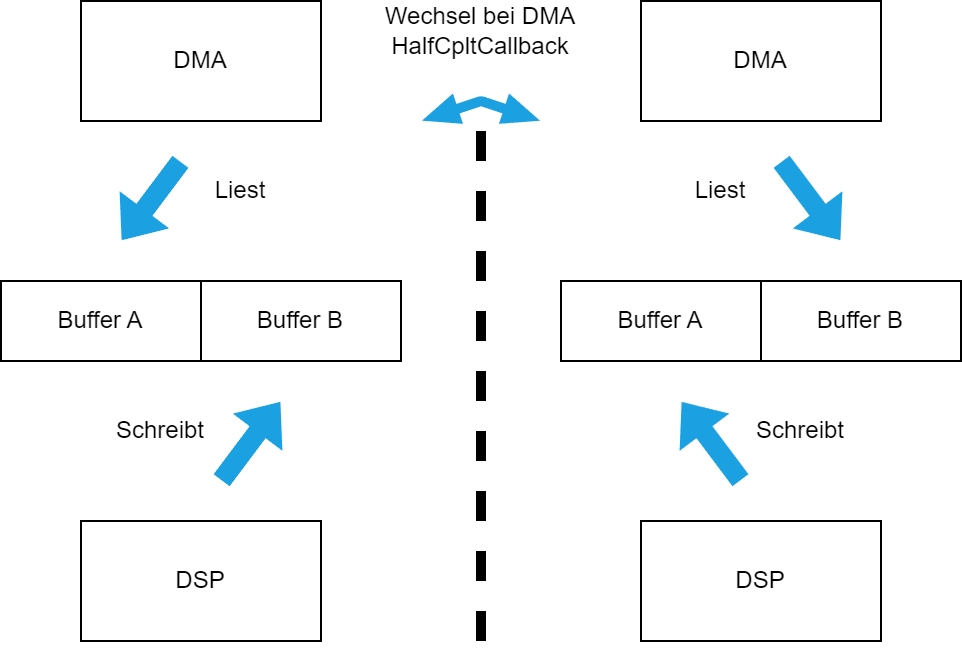
\includegraphics[width=0.6\textwidth]{images/08_durchfuehrung/audio/double_buffering.drawio.png}
	\caption{Double Buffering mit DMA und DSP}
	\label{fig:double_buffering}
\end{figure}


Bei I M A wird wird der Audiobuffer halbiert. %TODO: besser formulieren
Durch den Pointer \mintinline{c}|int16_t *outBufPtr| wird mit der DSP die Hälfte bearbeitet, die gerade nicht von der DMA übertragen wird.

In den Callback-Funktionen \mintinline{c}|HAL_I2S_TxHalfCpltCallback()| und \mintinline{c}|HAL_I2S_TxCpltCallback()| wird der Pointer auf die jeweilige Hälfte des Buffers, also auf (wie in  \textbf{\autoref{fig:double_buffering}} beschrieben:
\textbf{Buffer~A} und \textbf{Buffer~B}) gesetzt.


\inputminted[firstline=28, lastline=31]{c}{../../f401_sd_card_audio_codec_test/Core/Src/audio.c}

\inputminted[firstline=40, lastline=43]{c}{../../f401_sd_card_audio_codec_test/Core/Src/audio.c}


Diese Callbacks, werden systembedingt aufgerufen, sobald die DMA die erste Hälfte oder den gesamten Buffer übertragen hat. Sie eignen sich daher sehr gut um den Pointer zu setzen.

"Sobald das Flag \mintinline{c}|dma_dataReady == true| gesetzt ist, wird die nächste Bufferhälfte von der SD-Karte gelesen."

\subsubsection{PCM5102a und I2S}

Ein sehr weit verbreitetes Protokoll zur digitalen Audioübertragung ist I2S. Viele Codecs, so auch der PCM5102a, unterstützen dieses Protokoll.

I2S (Inter-IC Sound) ist ein Standard für die digitale Übertragung von Audiodaten zwischen integrierten Schaltkreisen (ICs). Es wurde entwickelt, um die Kommunikation von digitalen Audiodaten zwischen verschiedenen Komponenten wie Mikrofonen, DACs (Digital-Analog-Wandler) und ADCs (Analog-Digital-Wandler) zu ermöglichen. 

TODO: PCM5102a Signale erklären (SCK, LCK, BCK, DIN)

Der PCM5102a erkennt komfortablerweise die eingehende Samplerate anhand der Bitclock.
Anders als bei vielen Audio Codecs ist keine zusätzliche Konfiguration des Chips über ein Kommunikationsprotokoll, wie I2C notwending.
Somit fallen auch keine Treiber für diesen Chip an.

- Der Einfachheit halber, festgelegte Samplerate und nur Stereo Samples! vllt eher zum DSP/Playback Part


\subsubsection{SD Karte}

Durch den sehr begrenzter RAM-Speicher des NUCLEO F401re Boards , ist es notwendig die Daten in Echtzeit von der SD-Karte zu streamen. Das setzt bei Stereo PCM Dateien, mit den gängigen Parametern, eine bestimmte Datenrate \( R \) voraus:

\begin{itemize}
	\item Abtastrate (Sampling Rate): 44.100 Hz (44,1 kHz)
	\item Bit-Tiefe: 16 Bit
	\item Kanäle: 2 (Stereo)
\end{itemize}


Die Datenrate \( R \) berechnet sich aus:

\[
R = \text{Sampling Rate} \times \text{Bit-Tiefe} \times \text{Anzahl der Kanäle}
\]



\[
R = 44{,}100 \, \text{Hz} \times 16 \, \text{bit} \times 2
\]

\[
R = 1{,}411{,}200 \, \text{bit/s} \approx 0.168 \, \text{MB/s}
\]


Theoretisch hätte eine Implementierung des FATFS-Dateisystems über SPI ausreichen müssen, um diese Datenraten zu bewältigen. 

Um die SDIO-Schnittstelle in das FATFS-Dateisystem zu integrieren, mussten zunächst Treiber entwickelt werden. Diese Treiber mappen die üblichen Dateioperationen wie \mintinline{c}|f_open()|, \mintinline{c}|f_read()| usw. über die SPI-Schnittstelle.


In der Praxis stellte sich jedoch heraus, dass der Audiobuffer nicht schnell genug gefüllt worden ist, was starke Knackser und Störgeräusche mit sich gebracht hat.

\begin{wrapfigure}{r}{0.3\textwidth} % Increase the width of the figure environment
	\vspace{-30pt + 0.02\textwidth}
	\hspace{0.02\textwidth} % Add horizontal space
	\fbox{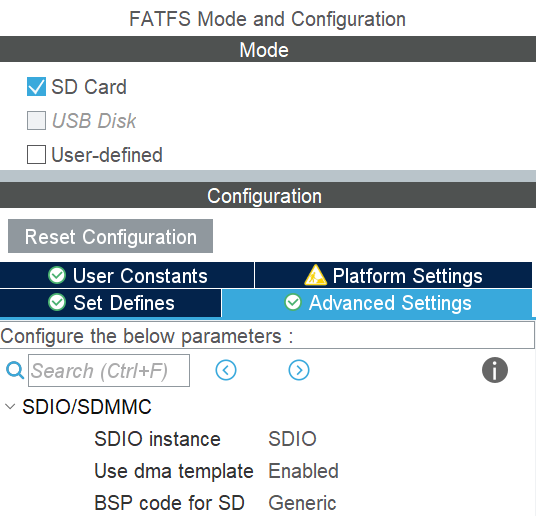
\includegraphics[width=0.28\textwidth]{images/08_durchfuehrung/audio/cubemx_sdio.png}}
	\caption{CubeMX FATFS SDIO Einbindung}
	\label{fig:cubemx_sdio}
\end{wrapfigure}

Dies erwies sich als äußerst vorteilhaft, da die SDIO-Implementierung zusammen mit FATFS direkt im Konfigurationstool von STM, \textbf{CubeMX}, ausgewählt werden kann. Die benötigten Treiber werden von CubeMX automatisch generiert und integrieren sich problemlos in das Dateisystem.

\subsubsection{Playback und Pitched Playback}


TODO Umsetzung im Code

CODE 

CODE 

CODE 

CODE 

CODE 

CODE 

CODE

CODE 


\subsubsection{Downsampling für die Verarbeitung von Audio durch das Neuronalen Netzes}
\label{sec:audio-downsampling}


